\section{Experiments}
\label{sec:experiments}

We will now return to the original question of the paper: Is planning
technology ready for applications in natural language generation? We
will tackle this question by evaluating the performance of several
planners on the NLG planning domains from the previous section.

We start with two experiments in the CRISP domain. First, we present a
scenario which focuses on the generation of referring expressions with
a tiny grammar (Section~\ref{sec:exper-1:-sent}); then we look at a
setting in which CRISP is used for surface realization with the XTAG
Grammar \citep{xtag01:_tr}, a large-scale TAG grammar of English
(Section~\ref{sec:exper-2:-sent-xtag}).

We then go through a series of experiments in the GIVE domain. We
start with a domain that is essentially Gridworld
(Section~\ref{sec:exper-2:-minim}), and then add positions that are
either not needed (Section~\ref{sec:experiment-3:-give}) or even
inaccessible (Section~\ref{sec:experiment-4:-give}). This series of
experiments is set up to illustrate what we perceive as the main
limitation of current off-the-shelf planners for our applications:
They spend a long time on computing all ground instances, even if most
of these instances are never used in the plan search.



\subsection{Experiment 1: Sentence generation (referring expressions)}
\label{sec:exper-1:-sent}

For the first experiment on sentence generation, we focus on the
generation of referring expressions, a problem that is usually handled
by the sentence planner if sentence planning and surface realization
are separated. We consider a series of sentence generation problems
which require the planner to compute a plan representing the sentence
``Mary likes the Adj$_1$ \ldots Adj$_n$ rabbit.''  Each problem
instance assumes a target referent $r$, which is a rabbit, and a
certain number $m$ of further rabbits $r_1,\ldots,r_m$ that are
distinguished by properties $P_1,\ldots,P_n$ with $n \leq m$. The
problem instance is set up such that $r$ has all properties except for
$P_i$ in common with each $r_i$. That is, all $n$ properties are
required to describe $r$ uniquely. The $n$ properties are realized as
$n$ different adjectives, in any order.  This setup allows us to vary
the plan length (a plan with $n$ properties will have length $n+4$)
and the universe size (the universe will contain $m+1$ rabbit
individuals in addition to the differently-typed individuals used to
encode the grammar).

\begin{figure}
  \centering
  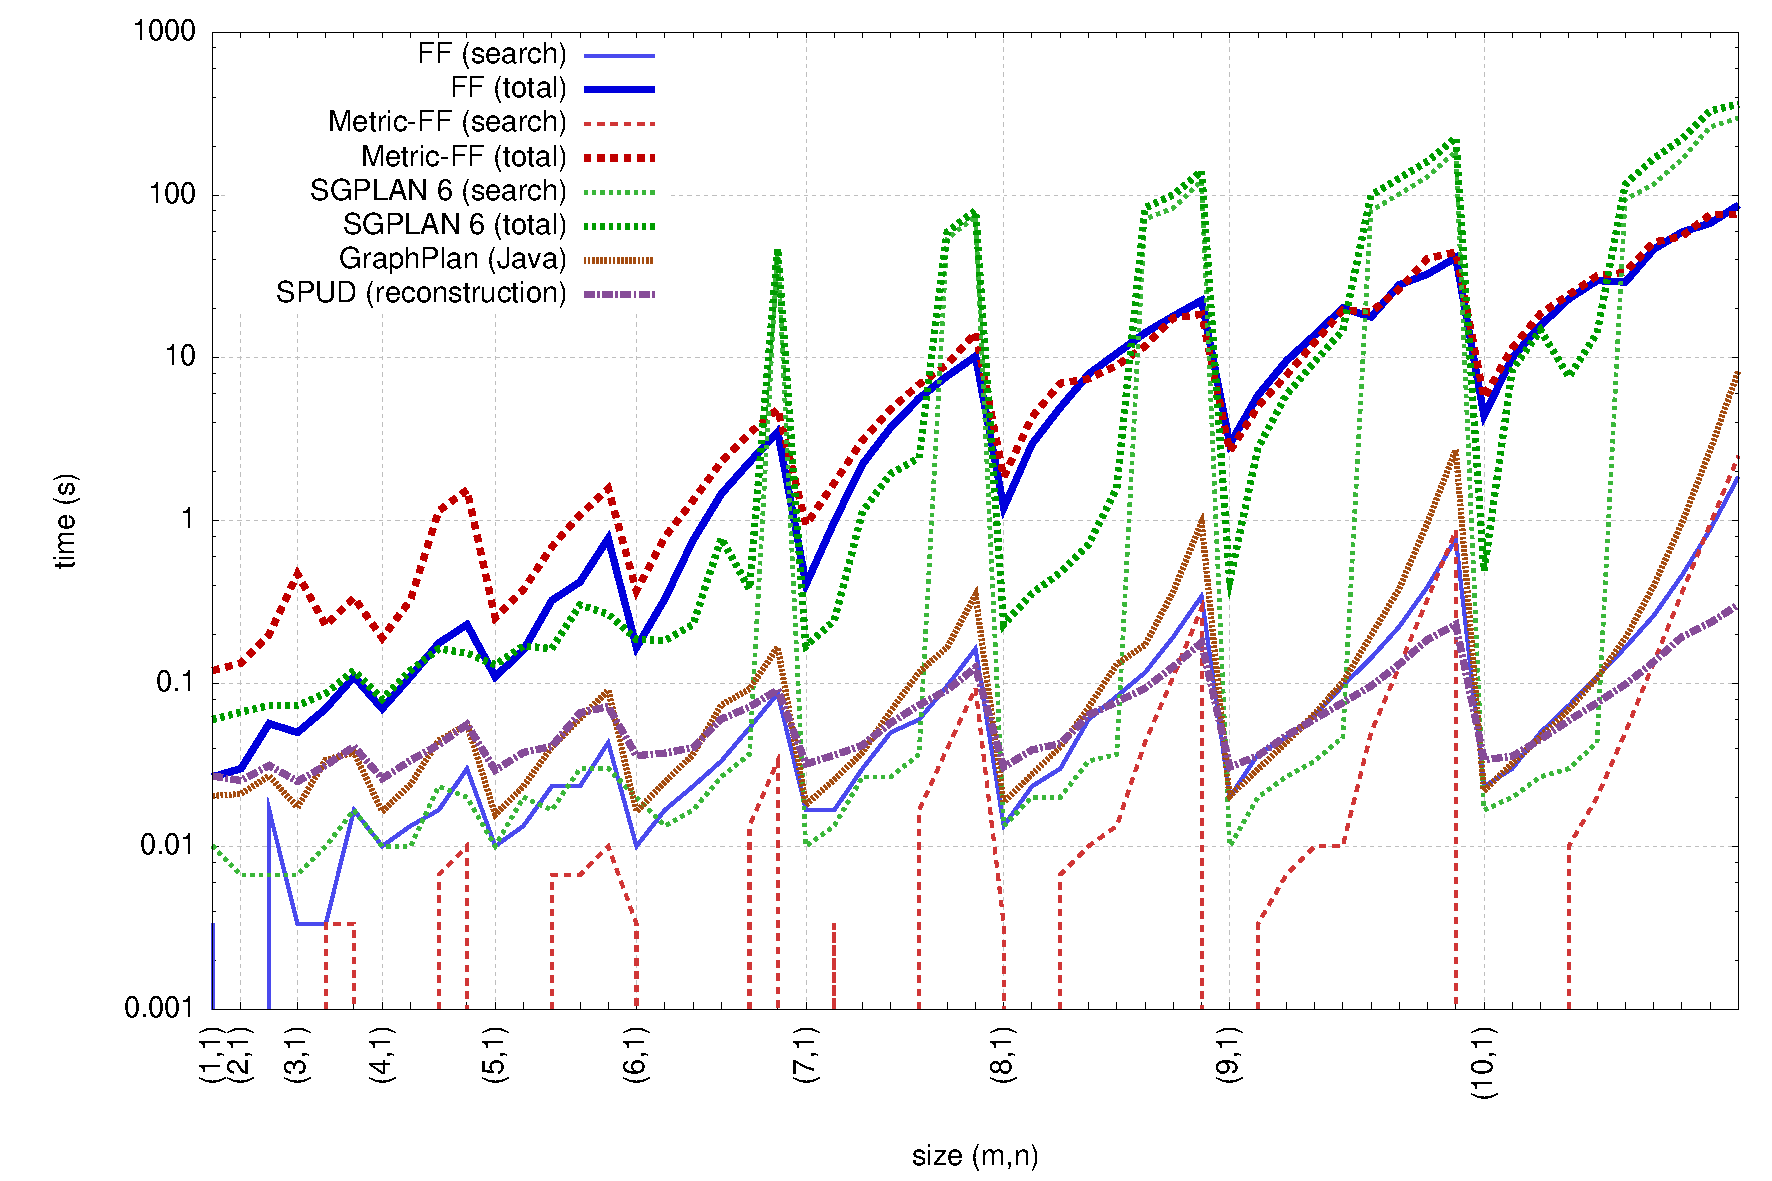
\includegraphics[width=\columnwidth]{data/modifiers-all}
  \caption{Results for the sentence generation domain. The
    horizontal axis represents parameters $(m,n)$ from $(1,1)$ to
    $(10,10)$ in lexicographical order. The vertical axis is the
    runtime in milliseconds.}
  \label{fig:runtimes-crisp}
\end{figure}

We converted these generation problem instances into planning problem
instances as described in Section~\ref{sec:domains}, and then ran
three different planners on them. We used the off-the-shelf planners
FF 2.3 \citep{HoffmannNebel01} and SGPLAN 5.2.2
\citep{hsu06:_new_featur_in_sgplan_for}, because they were highly
successful in the recent International Planning Competitions, and
support a fragment of PDDL with quantified and conditional effects,
which is necessary in our domain (see
Fig.~\ref{fig:white-rabbit-as-planning}). Common to both of these
planners is that they perform a preprocessing step in which all ground
instances of all predicates and actions are computed.  Furthermore, we
used an ad-hoc implementation of GraphPlan \citep{Blum1997} written in
Java which avoids the grounding preprocessing step and only computes
instances of actions and predicates by need, as they are actually
discovered when the planning graph is built. Our expectation was that
this planner would not be able to compete with FF or SGPLAN in terms
of search efficiency, but we were interested in comparing the
contribution of the prior grounding step on the planner performance.

The results of this experiment are shown in the graph in
Figure~\ref{fig:runtimes-crisp}.\footnote{All runtimes in
  Sections~\ref{sec:exper-1:-sent} and \ref{sec:exper-2:-sent-xtag}
  were measured on an AMD Opteron 8220 CPU running at 2.8 GHz, under
  Linux. FF 2.3 and Metric-FF were recompiled as 64-bit binaries. Java
  programs were executed under Java 1.6.0\_13 in 64-bit mode. They
  were allowed to ``warm up'', i.e. the JVM was given the opportunity
  to just-in-time compile the relevant bytecode by running the planner
  three times and discarding the runtimes before taking the actual
  measurements. All runtimes are averaged over three runs of
  the planners.} The input parameters $(m,n)$ are plotted in
lexicographic order on the horizontal axis, and the runtime is shown
in seconds on the vertical axis. These results reveal a number of
interesting insights. First, FF significantly outperforms SGPLAN in
this domain, sometimes by a factor of 10 or more. Second, FF's runtime
is dominated by its initial grounding step, in which it computes the
ground instances of all predicates and actions used in the planning
problem in order to avoid unnecessary instantiation during search.  In
particular, the ratio of grounding time to total runtime is generally
above 85\%, and rises to above 99\% at $m=11$, which is still a
relatively small universe for this application.\footnote{The
  ``grounding'' time reported here is what FF reports as ``time spent:
  instantiating action templates''.}

In our testing examples, the time spent by FF on grounding is so high
that it is consistently outperformed by our Java implementation of
GraphPlan, which only computes instances by need. Although FF is
consistently much faster as far as pure search time is concerned, our
results indicate that FF's performance is much more sensitive to the
domain size: if we fix $n=1$, FF takes 60 ms to compute a plan at
$m=1$, but 2.4 seconds to compute the same plan at $m=10$. By
comparison, our GraphPlan implementation takes 30 ms at $m=1$ and
still only requires 50 ms at $m=10$. Conversely, GraphPlan's runtime
grows much faster with the plan size (i.e., with growing values of $n$
for a fixed $m$). Larger, but still realistically-sized, instances of
the sentence generation problem are still problematic for all the
planners we tested.



\subsection{Experiment 2: Sentence generation (XTAG)}
\label{sec:exper-2:-sent-xtag}

The first experiment already gives us some initial insights into the
appropriateness of planning for the sentence generation domain: On the
examples we looked at, search times were low, but FF and SGPLAN spend
a lot of time on the initial grounding step.  However, one weakness of
this experiment is that it uses a tiny grammar, consisting of just
those 12 lexicon entries that are needed for the experiment. While the
grounding problem can only get worse with larger grammars, the
experiment by itself does not allow us to make clear statements about
the search efficiency.

To address this problem, we ran a second sentence generation
experiment. This time, we used the XTAG Grammar \citep{xtag01:_tr}, a
large-scale TAG grammar of English. XTAG contains lexicon entries for
about 17,000 uninflected words using about 1100 different elementary
trees. Although XTAG does not contain semantic information, it is
possible to automatically equip the lexicon entries with inferred
semantic representations based on the words in the lexicalized
elementary tree. The result is a highly ambiguous grammar: The most
ambiguous word, ``ask'', is the anchor of 314 lexicon entries.

In our experiment, we were especially interested in two
questions. First, how would the planners handle the search problem
involved in generating with such a large and ambiguous grammar?
Second, would it be harder to generate sentences containing verbs with
multiple arguments, given that verbs with more arguments lead to
actions with more parameters and therefore more instances? To answer
these questions, we generated sentences of the form ``S and S and
\ldots and S'', where each S was a sentence; we called the number of
sentences in the conjunction $n$. Each S was a sentence of the form
``the businessman sneezes'', ``the businessman admires the girl'', or
``the businessman gives the girl the book''---that is, they varied in
the number $k$ of syntactic arguments the verb expects (1 for the
intransitive verb ``sneeze'', 2 for the transitive verb ``admire'',
and 3 for the ditransitive verb ``give''). This means that the output
sentence for parameters $n$ and $k$ contained $n(2k+2)-1$ words. The
instances were set up in such a way that the generation of referring
expressions was trivial, so this experiment was purely a surface
realization task. To achieve reasonable performance, we only generated
planning operators for those elementary trees for which all predicate
symbols in the semantic representation also appeared in the knowledge
base.

\begin{figure}[t]
\subfloat[$k=1$]{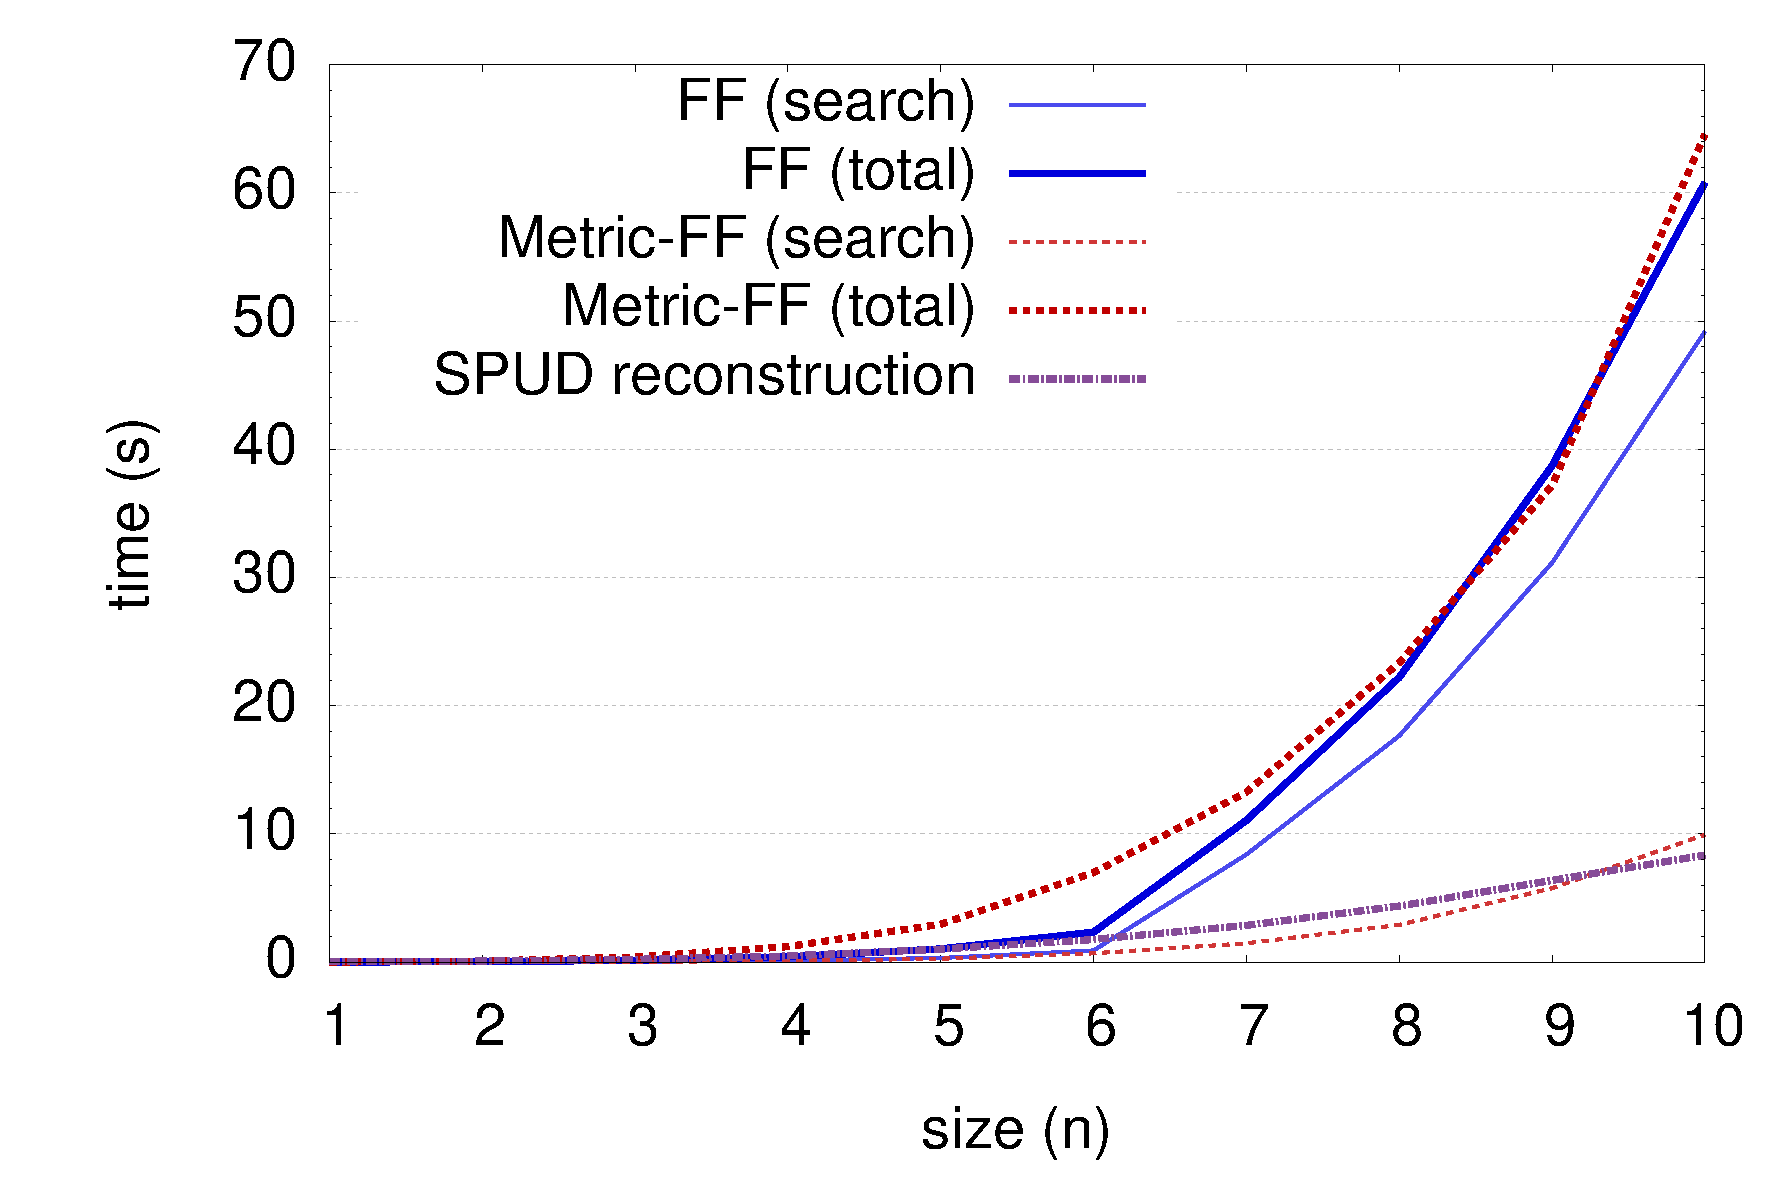
\includegraphics[width=8cm]{data/xtag-k1.pdf}}
\subfloat[$k=2$]{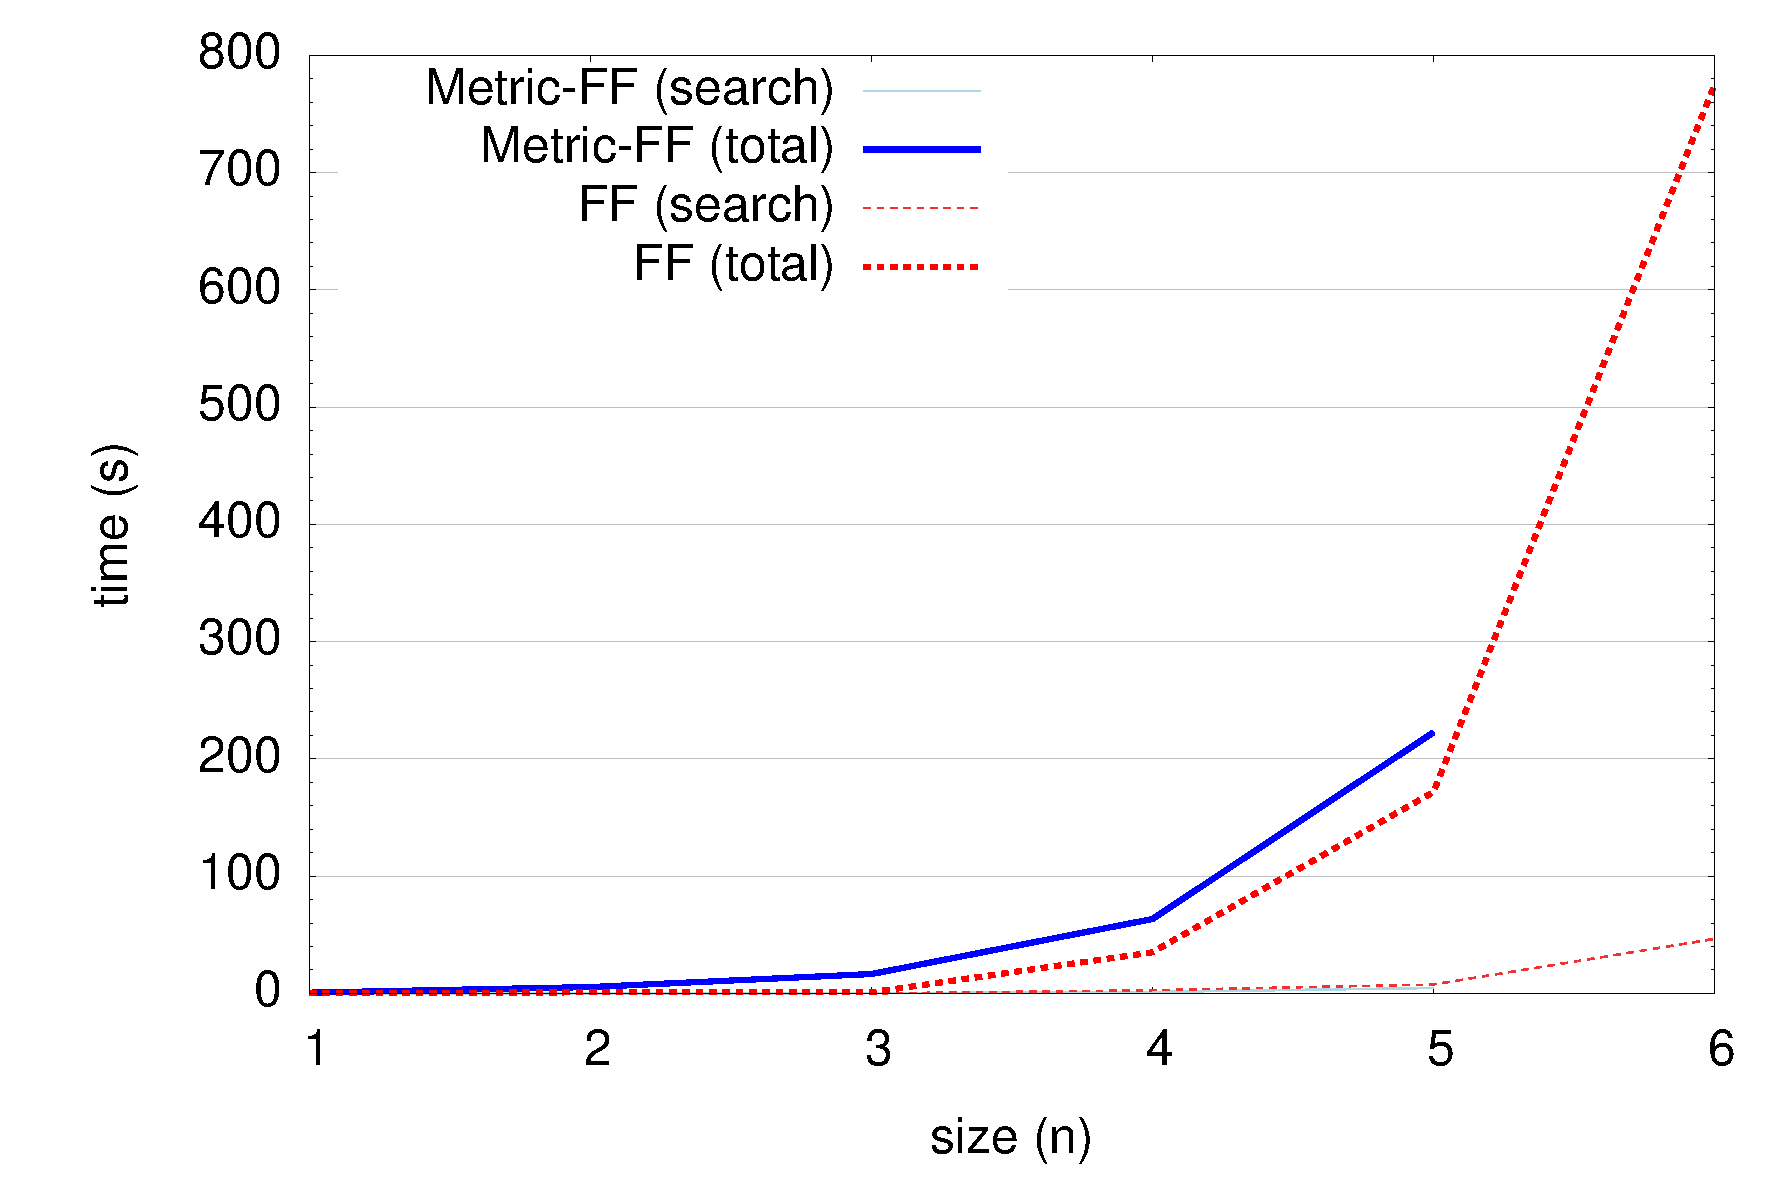
\includegraphics[width=8cm]{data/xtag-k2.pdf}}
  \caption{Results for the XTAG experiment, at $k=1$ and $k=2$.}
  \label{fig:xtag-graph}
\end{figure}

Fig.~\ref{fig:xtag-graph} reports the runtimes we measured in this
experiment for FF. Because the computations in this experiment were
very memory-intensive, we recompiled FF 2.3 as a 64-bit binary. We
also ran the experiments with a 64-bit version of Metric-FF; although
our planning problem is purely sequential and not metric, Metric-FF
avoids a bug which caused FF 2.3 to switch to a best-first search
strategy beyond a certain point; the jump in runtime is clearly
visible in the figure. We did not run this experiment with SGPLAN
because we didn not have access to a 64-bit version of either SGPLAN
5.2.2 or SGPLAN 6; some initial experiences with the 32-bit version
indicate that SGPLAN switches to FF's best-first strategy even for
small problem instances, and thus would be slower than the versions of
FF we reported here. We also do not report runtimes for our Java
implementation of Graphplan, because it was unusuably slow for serious
problem instances: For $k=1$ and $n=3$, it already took over two
minutes, and it exceeded its memory limit of 16 GB for
$n>3$. \todo{compare to SPUD reconstruction here}

There are a number of observations we can make in this
experiment. First of all, the experiment confirms that FF's Enforced
Hill-Climbing search strategy works very well for the sentence
generation task: Although we are now generating with a large grammar,
FF generates a 39-word sentence ($k=1,n=6$) in under a second of
search time. This efficiency is a direct result of this particular
search strategy: Whenever FF falls back to the best-first strategy,
runtimes become much slower (compare the graphs for FF 2.3 and
Metric-FF). Second, FF's runtime is still dominated by the
preprocessing stage. For instance, Metric-FF spends about 10 seconds
on search for $k=1,n=10$, compared to its total runtime of about 65
seconds. This effect becomes more pronounced as we increase $k$: For
$k=2$, we reach 65 seconds of total runtime at $n=4$, but here
Metric-FF only spends about a second on search. For $k=3$, neither FF
nor Metric-FF were able to solve any of the input
instances. \todo{bla} This is to be expected, given that the planning
operators for the verbs have $k+2$ parameters (see
Fig.~\ref{fig:white-rabbit-as-planning}), and thus the number of
action instances grows by a factor of the universe size every time we
increase $k$ by one. A planner which computes all ground instances of
the operators thus takes exponential time in $k$ for preprocessing.




\subsection{Experiment 2: Minimal GIVE worlds}
\label{sec:exper-2:-minim}

In the second experiment, we evaluate the performance of the planners on
problems arising in the GIVE domain. We construct a series of test worlds,
similar to the one illustrated in Figure~\ref{fig:give-minimal}. These
worlds consist of a $2n$ by $h$ grid of positions, such that there are
buttons at positions $(2i-1,1)$ and $(2i,h)$ for $1 \leq i \leq n$. The
player starts in position $(1,1)$ and must press all the buttons
to successfully complete the game. The world is generated as a GIVE world
description, and then automatically converted into a planning problem by
the GIVE software. For instance, Figure~\ref{fig:give-planning} shows some
of the actions available in the GIVE domain in PDDL syntax.

\begin{figure}[t]
  \centering
  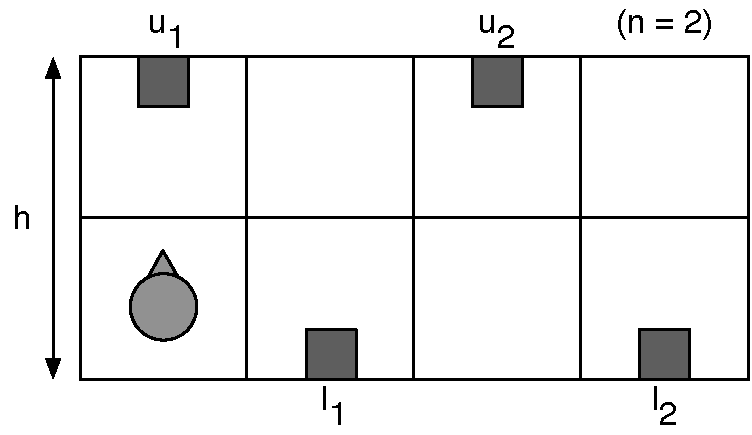
\includegraphics[width=0.5\columnwidth]{pic-buttons}
  \caption{Minimal GIVE world.}
  \label{fig:give-minimal}
\end{figure}

Results for the $h=20$ case, with $n$ ranging from $1$ to $40$, are shown
in Figure~\ref{fig:give-runtime-minimal}. The most obvious result is that
FF is unable to solve any problems beyond $n=13$ on our experimentation
machine within the memory limit of 1 GB. SGPLAN, on the other hand, solves
instances beyond $n=40$ without major problems. In this case, our
implementation of GraphPlan is unable to find any of these plans. The time
spent on grounding is not a major factor in either planner, probably
because the planners need more time to actually compute the plan---for
instance, the optimal plan for the problem $n=40$ has a length of about
1600 steps. As a concrete example, the following is a minimal plan for the
case of a $2$ by $2$ grid with $2$ buttons for the player to press (i.e.,
$n=1$, $h=2$):

\begin{enumerate}
\item $\mathsf{move}(\mathsf{pos\_1\_1},\mathsf{pos\_1\_2}, \mathsf{north})$,
\item $\mathsf{manipulate}\textsf{-}\mathsf{u1}\textsf{-}\mathsf{off}\textsf{-}\mathsf{on}(\mathsf{pos\_1\_2})$,
\item $\mathsf{turn}\textsf{-}\mathsf{right}(\mathsf{north}, \mathsf{east})$,
\item $\mathsf{move}(\mathsf{pos\_1\_2}, \mathsf{pos\_2\_2},
  \mathsf{east})$,
\item $\mathsf{turn}\textsf{-}\mathsf{right}(\mathsf{east}, \mathsf{south})$,
\item $\mathsf{move}(\mathsf{pos\_2\_2}, \mathsf{pos\_2\_1}, \mathsf{south})$,
\item $\mathsf{manipulate}\textsf{-}\mathsf{l1}\textsf{-}\mathsf{off}\textsf{-}\mathsf{on}(\mathsf{pos\_2\_1})$.
\end{enumerate}


\begin{figure}[t]
  \centering
  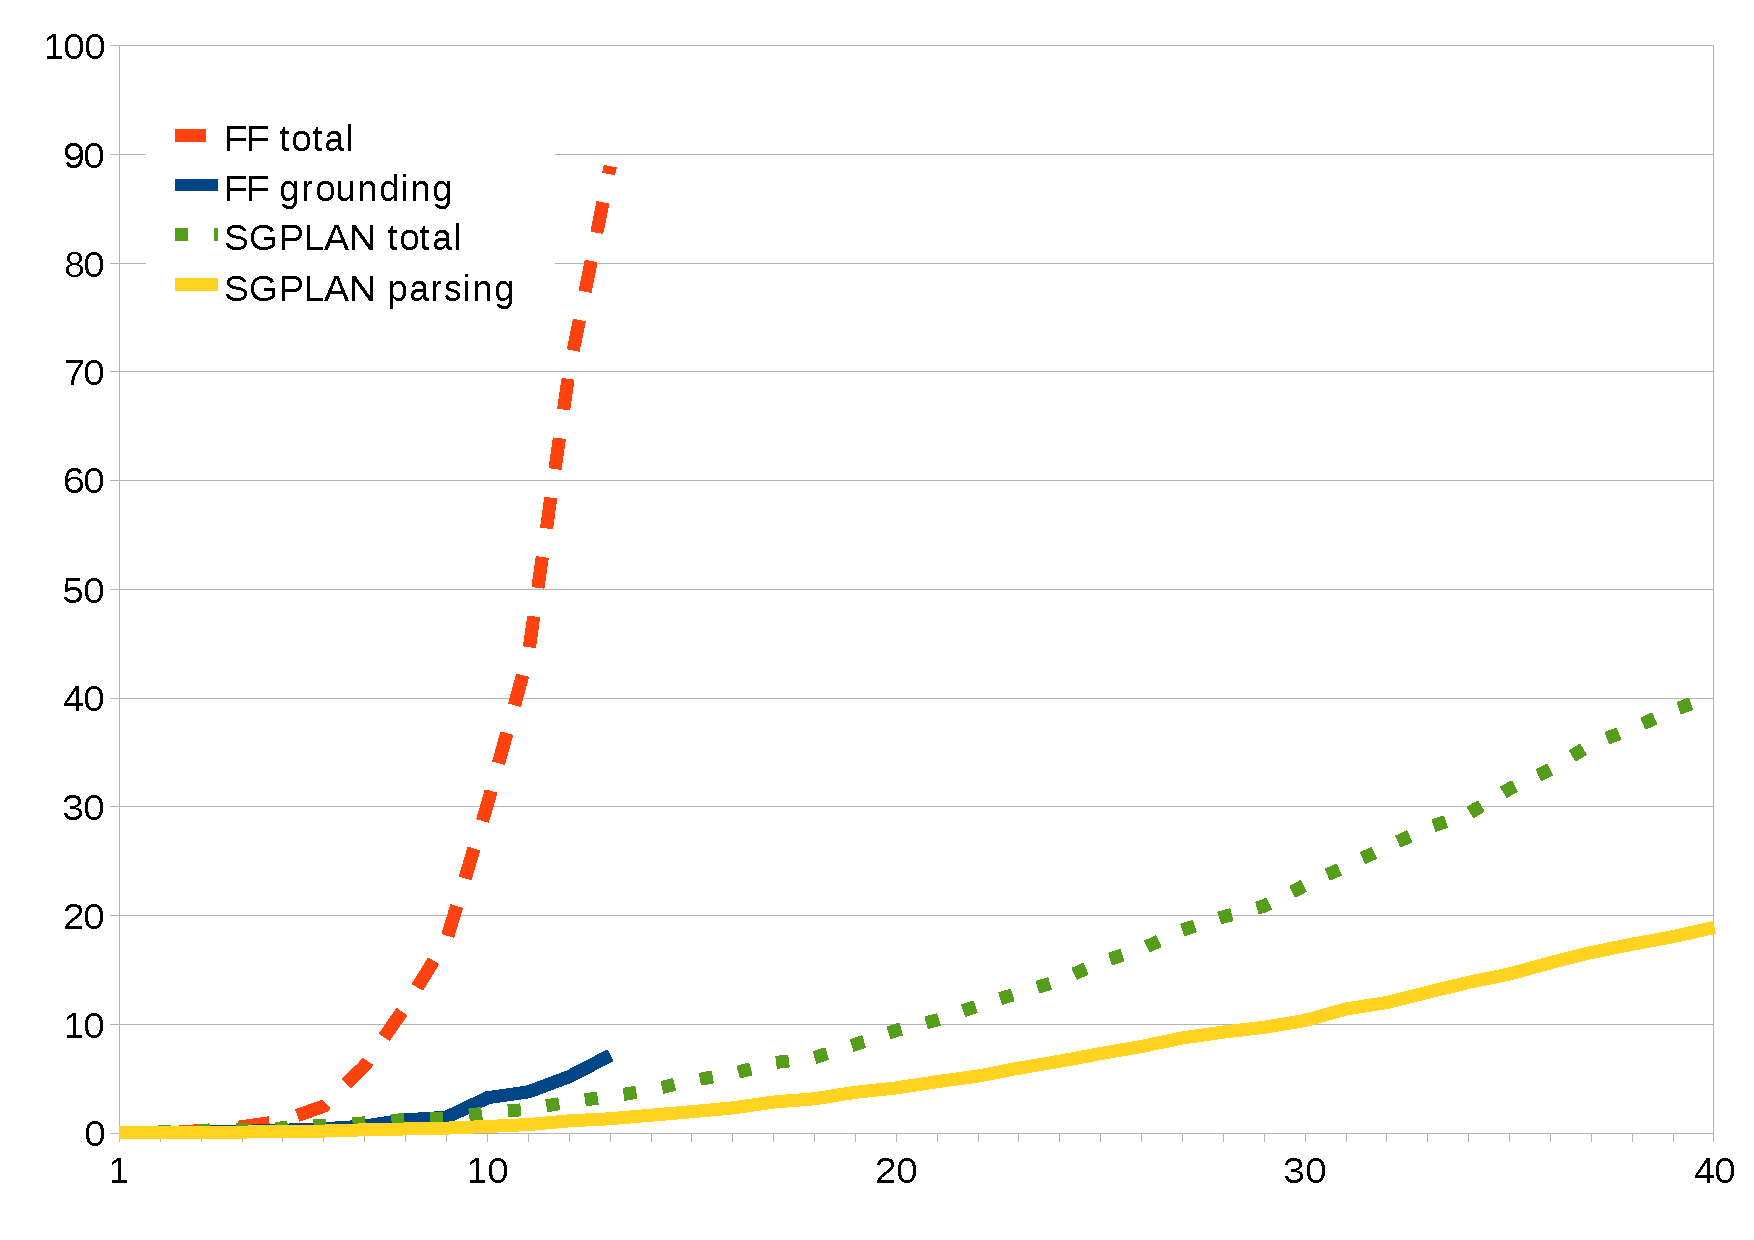
\includegraphics[width=0.75\columnwidth]{graph-exp2}
  %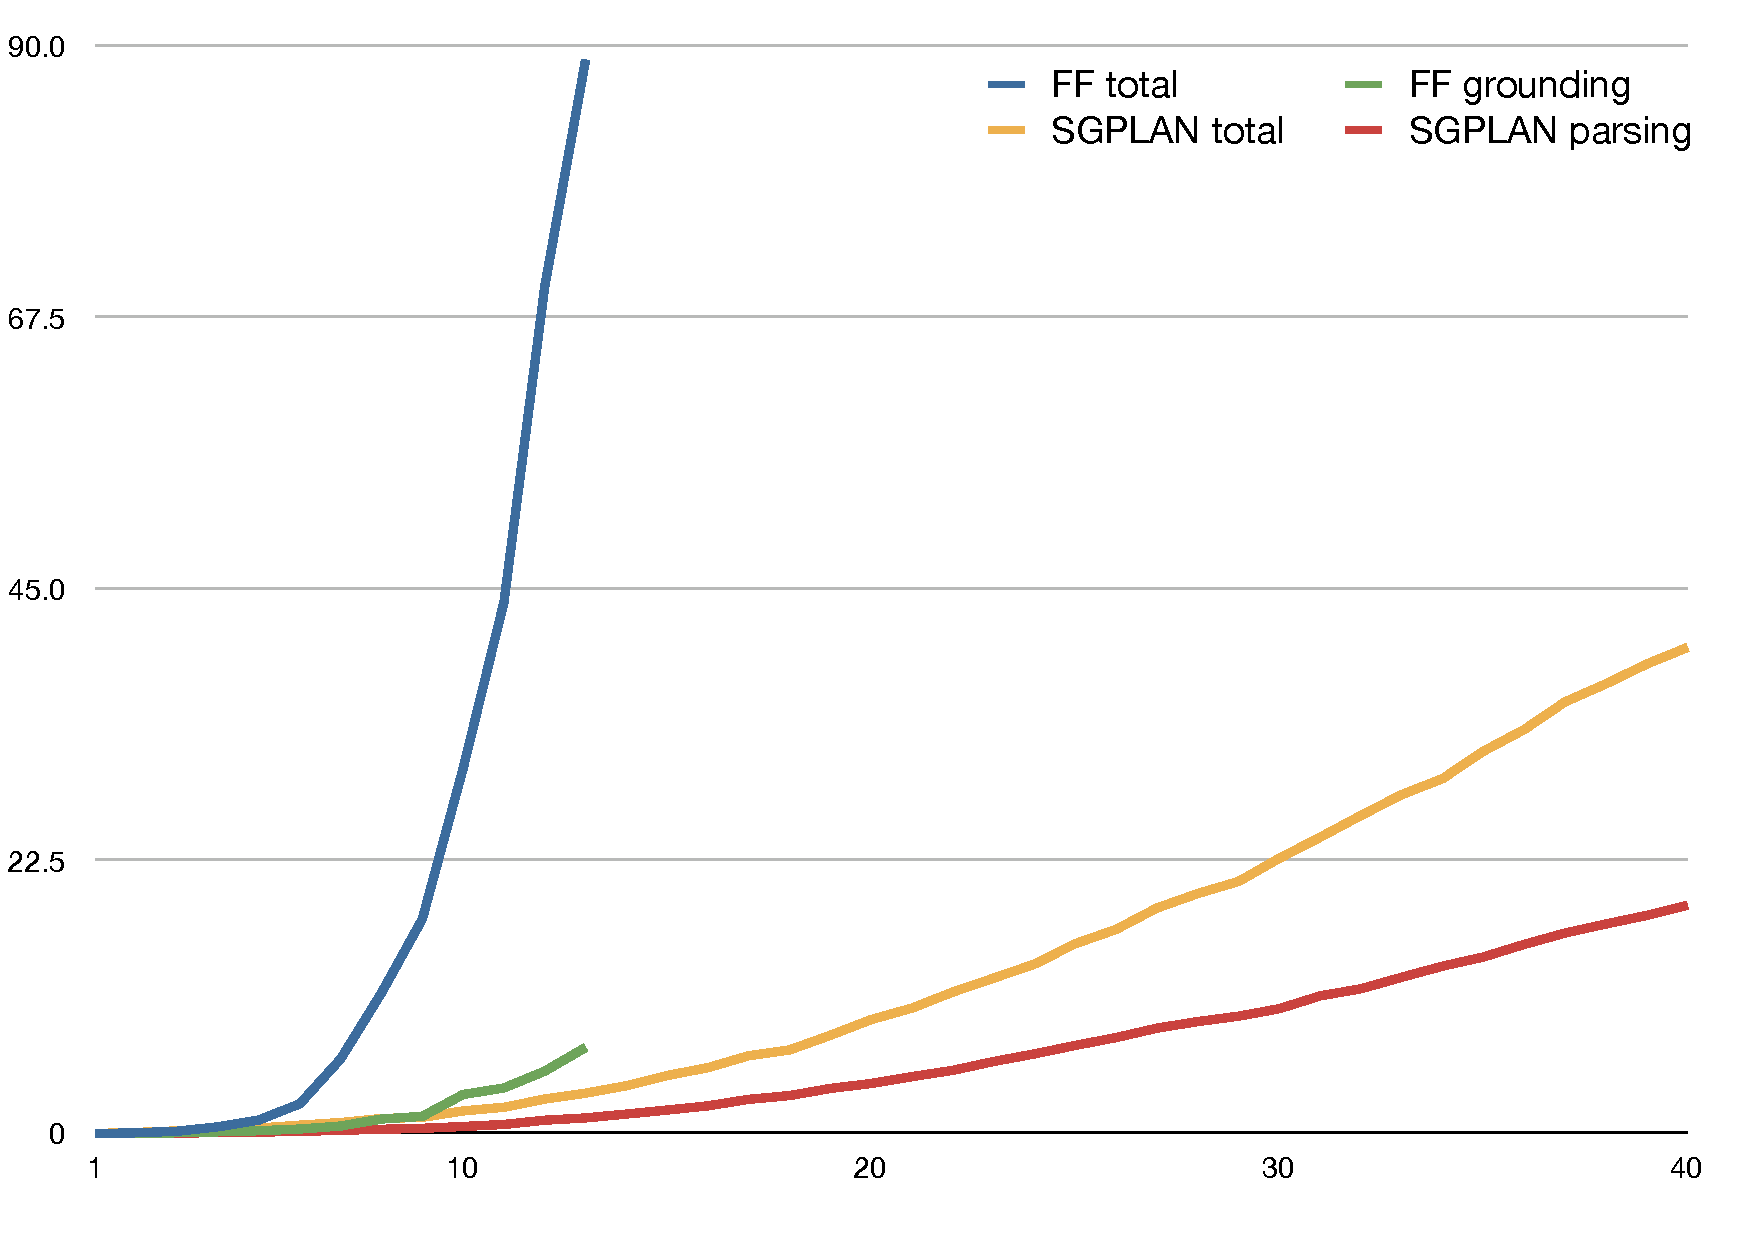
\includegraphics[width=1\columnwidth]{pic-runtime-buttons}
  \caption{Results on the minimal GIVE
    domain for $h=20$. The horizontal axis is $n$. The vertical axis
    is the runtime in seconds.}
  \label{fig:give-runtime-minimal}
\end{figure}


\subsection{Experiment 3: GIVE worlds with extra positions}
\label{sec:experiment-3:-give}

In the third experiment, we vary the structure of the GIVE world in order
to judge the effect that universe size has on the planning problem in this
domain. Starting with the ordinary GIVE world described in Experiment~2, we
extend the world map by adding another $w$ by $h$ empty ``junk'' positions
to the right of the minimal world, as shown in Figure~\ref{fig:give-junk}.
These new positions are not actually required in any plan, but extend the
size of the state space and approximate the situation in the actual GIVE
domain where most grid positions are never used. We leave the initial state
and goal untouched. As before, we generate a GIVE world description and
then convert it into a planning problem in PDDL.

\begin{figure}[t]
  \centering
  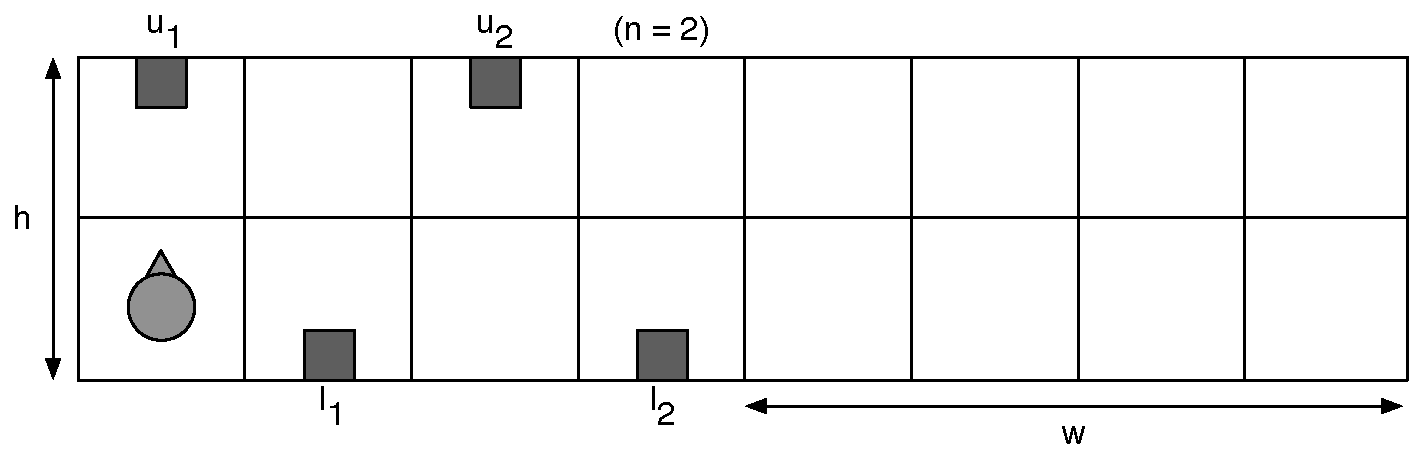
\includegraphics[width=0.80\columnwidth]{pic-empty-buttons}
  \caption{GIVE world with extra ``junk'' positions.}
  \label{fig:give-junk}
\end{figure}

Results for the $h=20$, $n=5$ case with $w$ ranging from $1$ to $70$ are
shown in Figure~\ref{fig:give-runtime-junk}. As in Experiment~2, FF again
runs out of memory, this time at $w=17$, while SGPLAN easily solves inputs
beyond $w=70$. As in Experiment~2, our implementation of GraphPlan is
unable to generate any of these plans. Unlike Experiment 2, however, both
FF and SGPLAN now spend a substantial proportion of their time on
grounding. In SGPLAN, this translates to a ``parsing time'' (which we
assume includes grounding) which grows from 180 ms to 21.7 seconds as $w$
grows from $1$ to $75$. The rest of the runtime, which also includes the
search time, only grows from 400 ms to 2.3 seconds. This difference is
particularly dramatic given that the actual optimal plan in each case is an
identical plan of about 100 steps (i.e., the one we would have found in
Experiment 2 for the $h=20$, $n=5$ case). The planning times for these
instances are also concerning since times over a couple seconds will
negatively affect the overall response time of the system, which must react
in real time to user actions.

\begin{figure}[t]
  \centering
  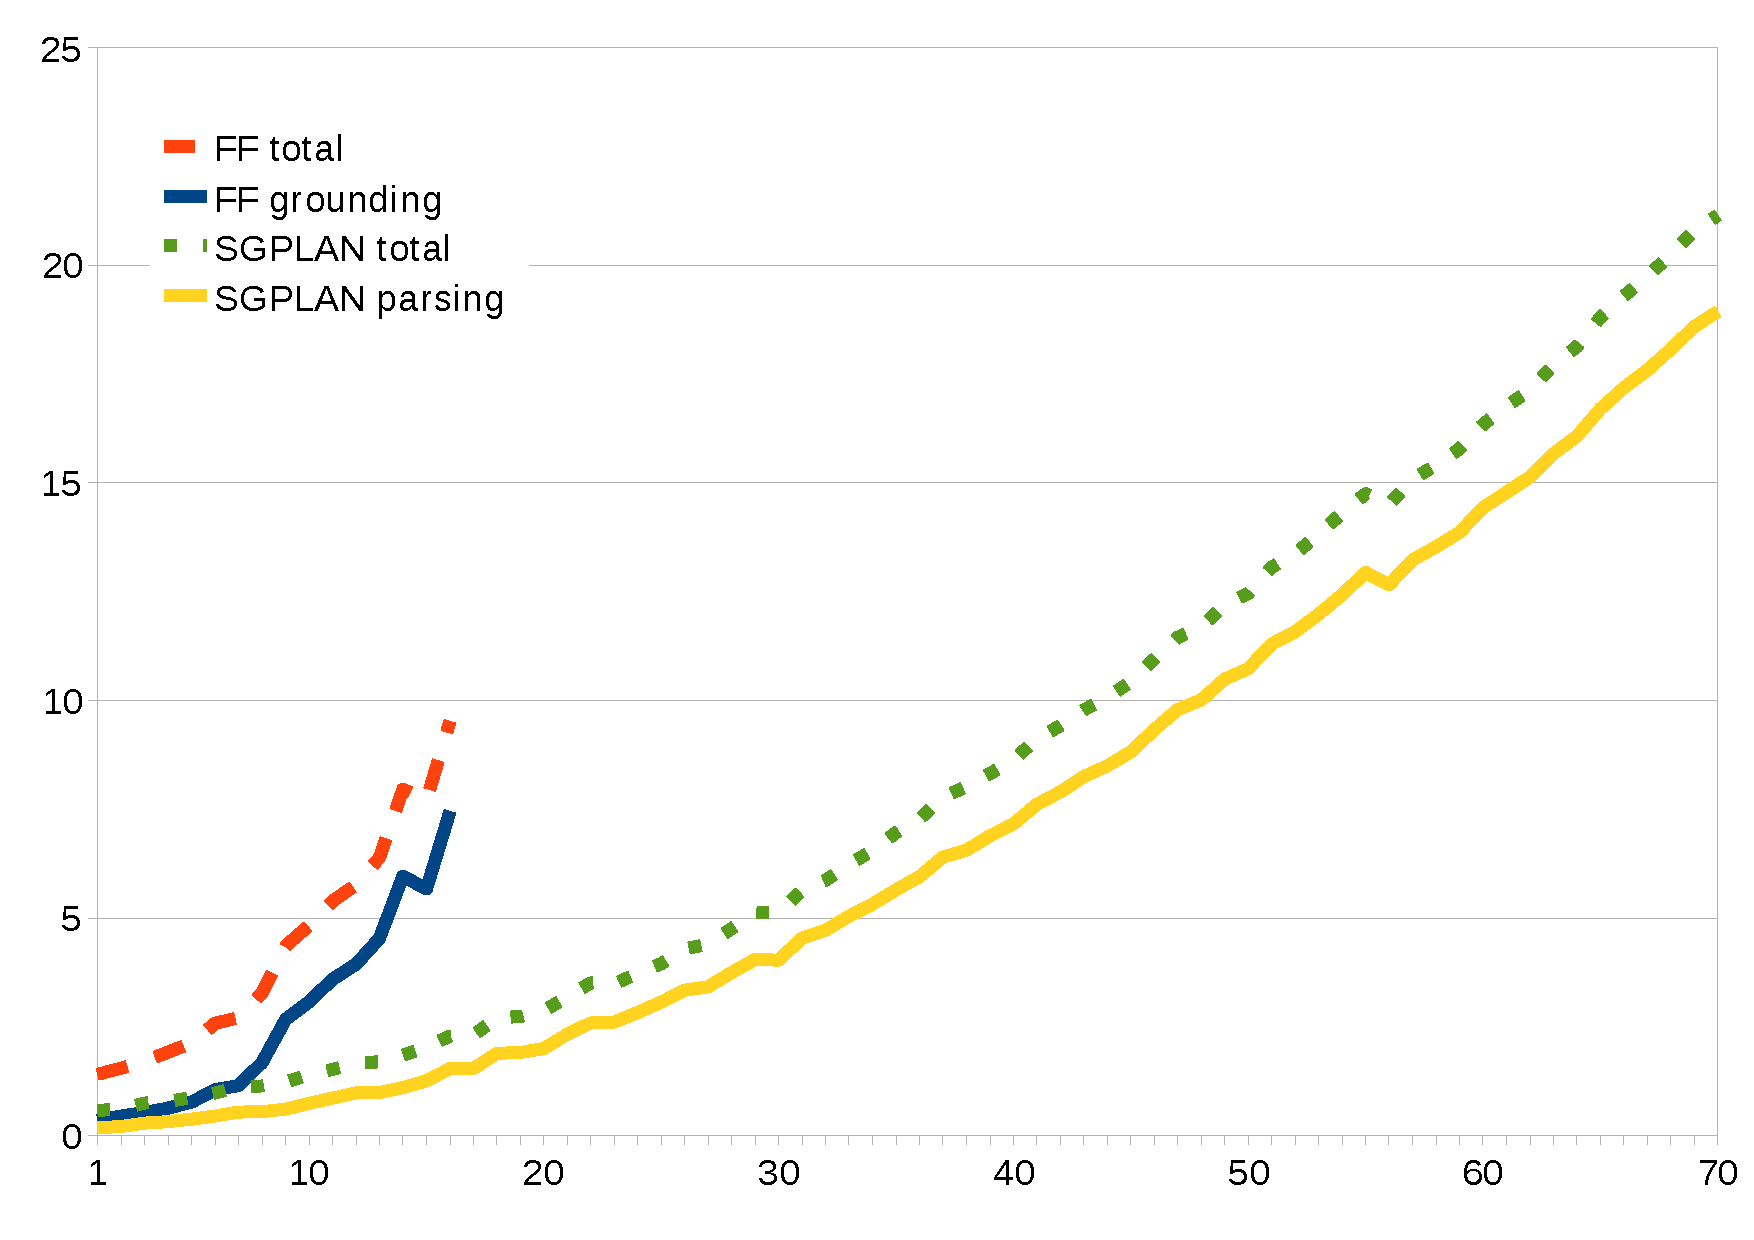
\includegraphics[width=0.75\columnwidth]{graph-exp3}
  %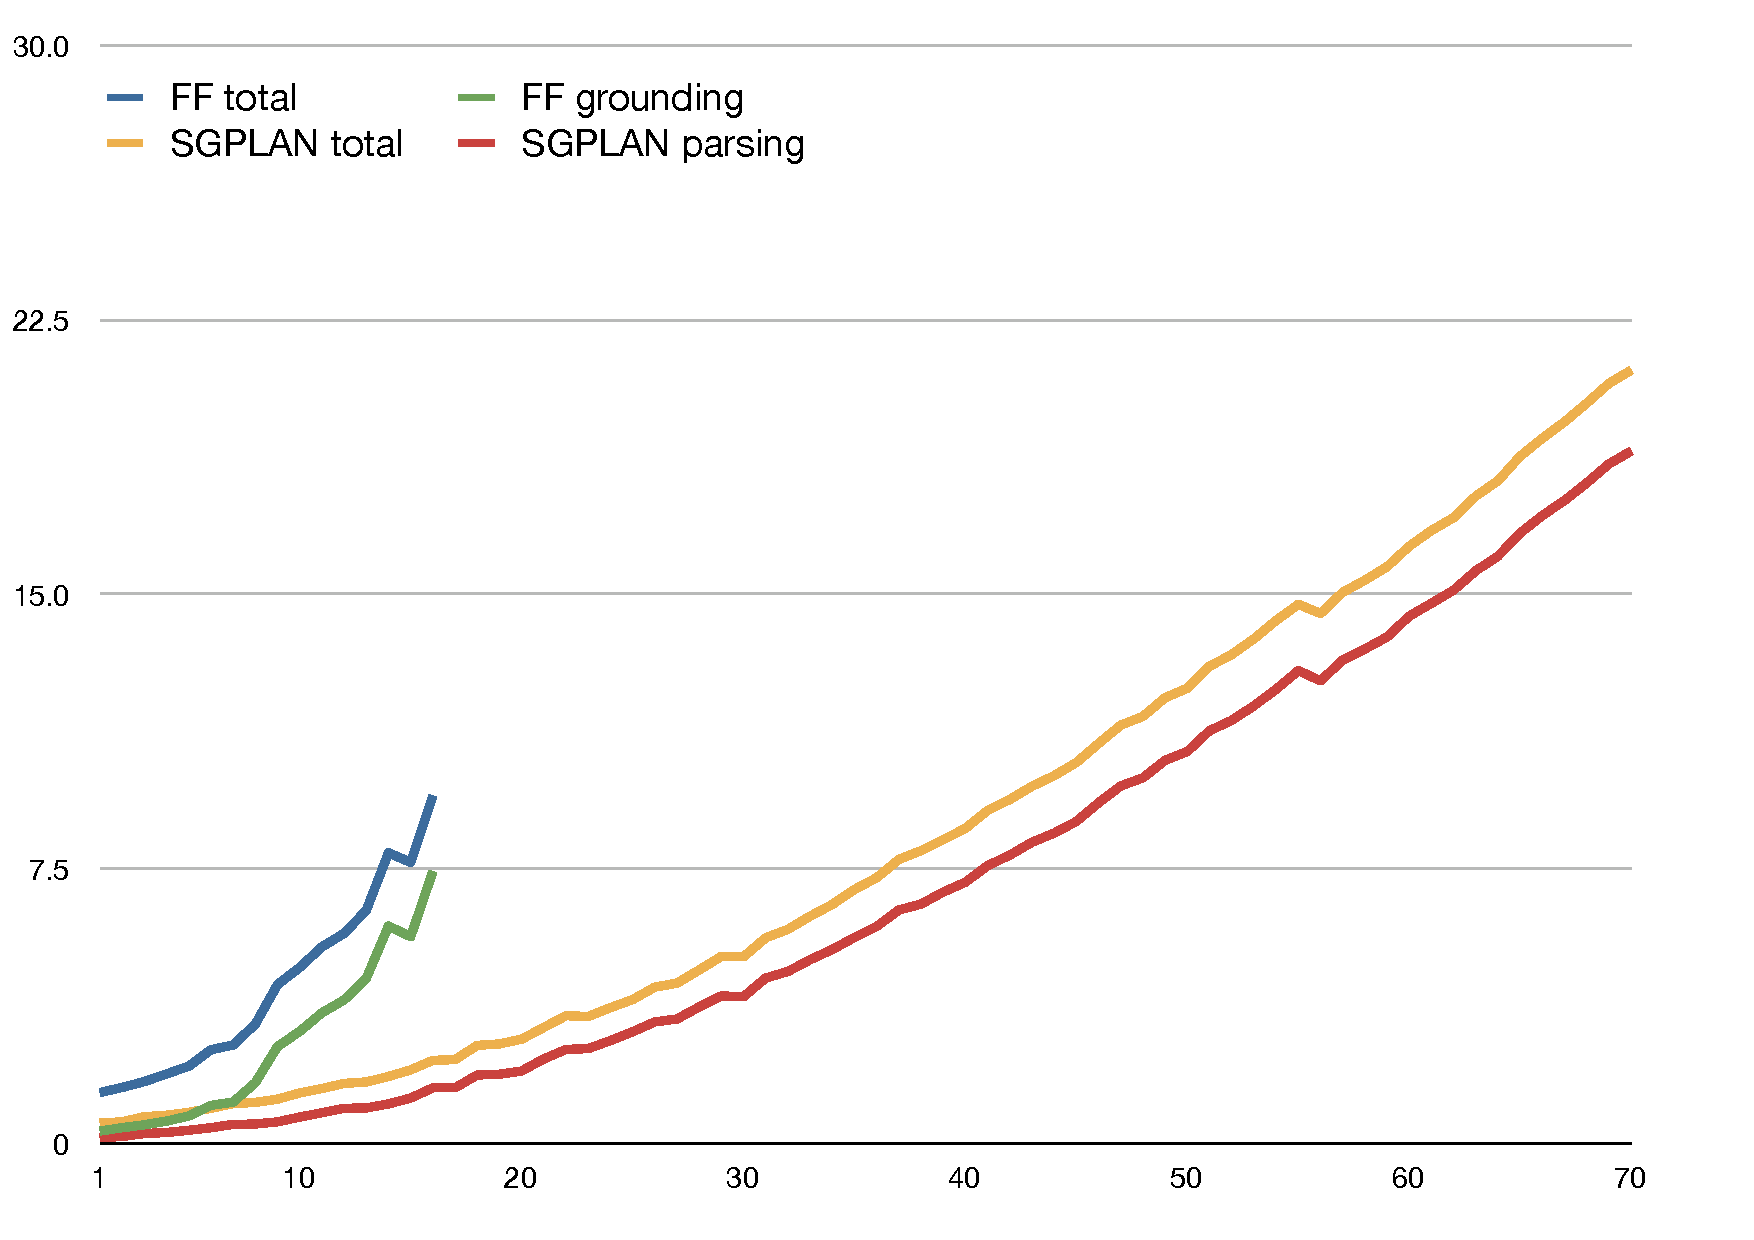
\includegraphics[width=1\columnwidth]{pic-runtime-empty-world}
  \caption{Results on the GIVE domain with junk
    positions for $h=20$ and $n=5$. The horizontal axis is $w$.
    The vertical axis is the runtime in seconds.}
  \label{fig:give-runtime-junk}
\end{figure}


\subsection{Experiment 4: GIVE worlds with inaccessible positions}
\label{sec:experiment-4:-give}

In the final experiment, we consider a variation on the GIVE worlds from
Experiment~3. As before, we begin with a base grid of $2n$ by $h$
positions, with buttons at positions $(2i-1,1)$ and $(2i,h)$ for $1 \leq i
\leq n$. We then generate a second grid of $w$ by $h$ positions and place
an additional button in this grid. Unlike Experiment~3, the second grid
does not extend the first grid but is ``disconnected'' so its positions are
inaccessible from the first grid, as shown in
Figure~\ref{fig:give-junk-nosoln}. Since the geometry of the grid makes it
impossible to construct a plan for pressing all the buttons in the world,
we instead investigate the time it takes a planner to arrive at the
conclusion that the problem cannot be solved.

Results for the $h=20$, $n=5$ case with $w$ ranging from 1 to 50 are shown
in Figure~\ref{fig:give-runtime-nosoln}.\footnote{FF and SGPLAN do
 not display runtimes when they fail to construct a plan so an external timing
 program was used to generate these results.}
In this case, the runtimes for FF rise sharply around $w=28$, producing
times that are unacceptable for an NLG system in practice. FF is unable
to complete problem instances above $w=35$. SGPLAN, by comparison, performs
exceptionally well and is able to complete problems instances up to $w=50$
in about 0.3 seconds and $w=80$ in about 0.6 seconds. These results
demonstrate that SGPLAN has a significant advantage over FF in this
experiment. 
%Our implementation of GraphPlan is unable to complete any of
%these problem instances.

\begin{figure}[t]
  \centering
  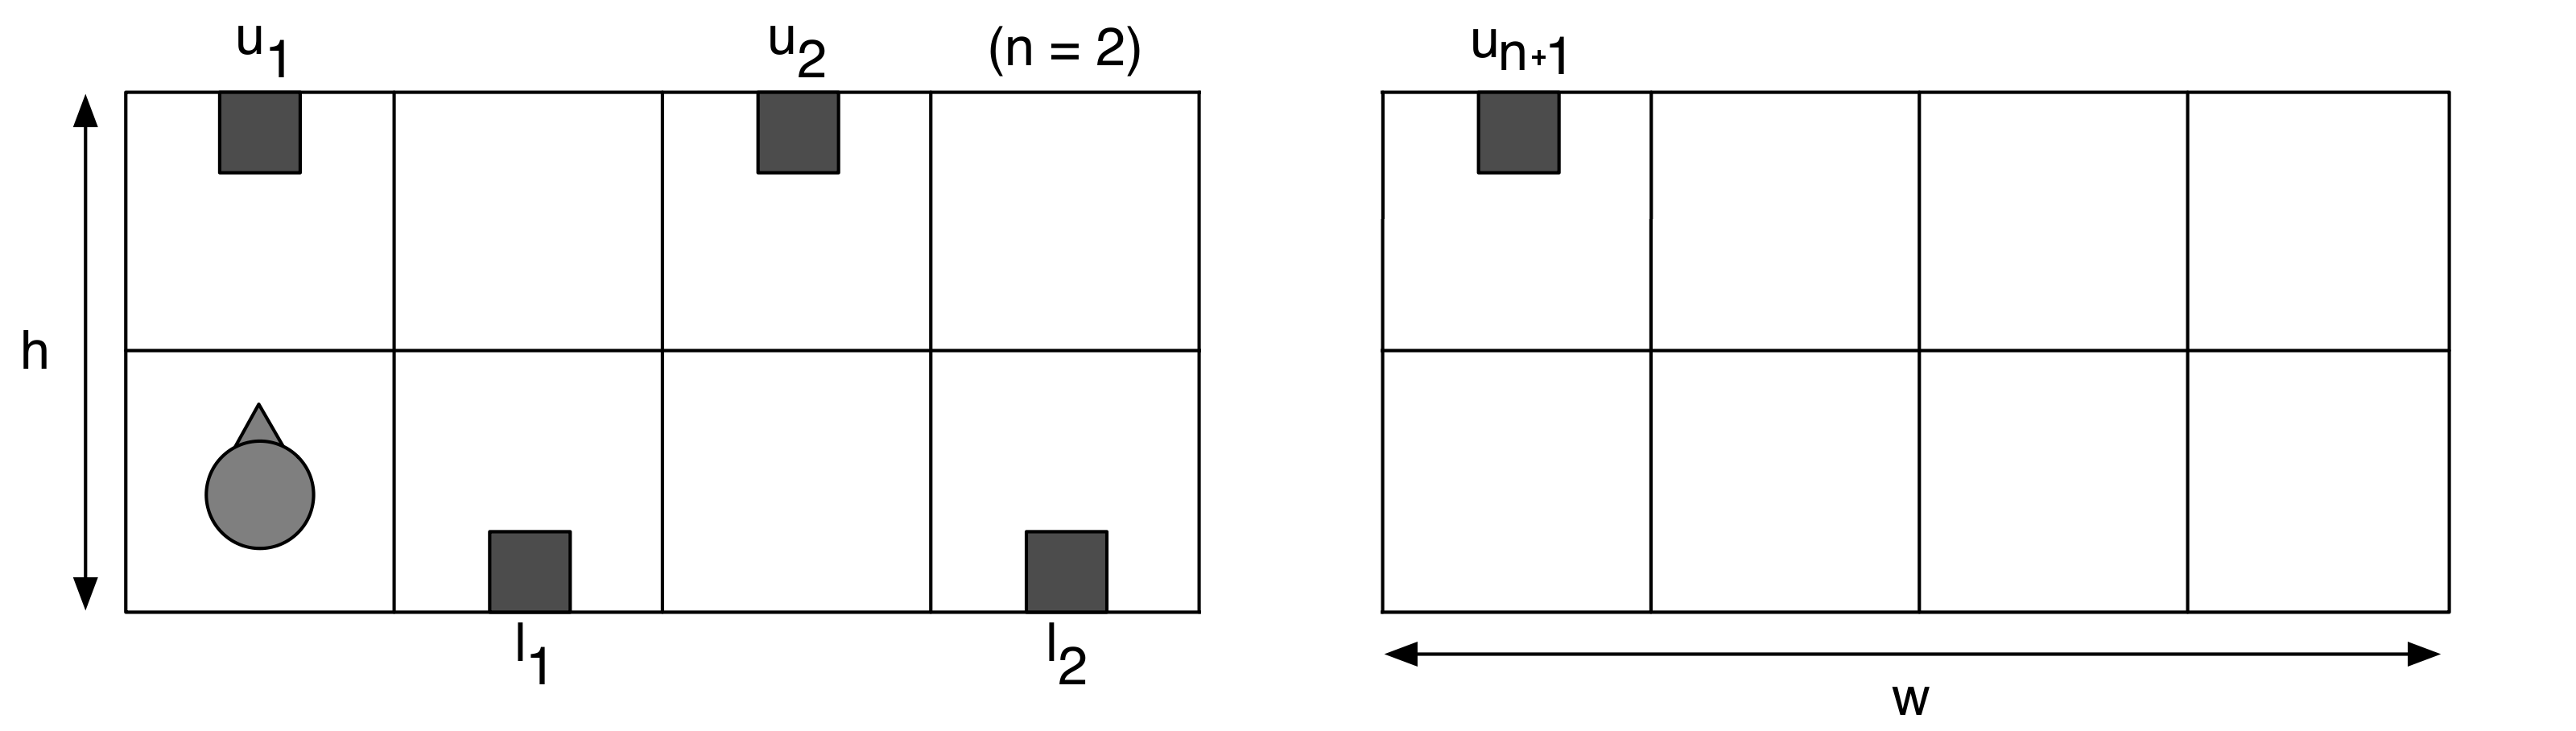
\includegraphics[width=0.85\columnwidth]{pic-empty-inaccessible}
  \caption{GIVE world with inaccessible positions.}
  \label{fig:give-junk-nosoln}
\end{figure}

\begin{figure}
  \centering
  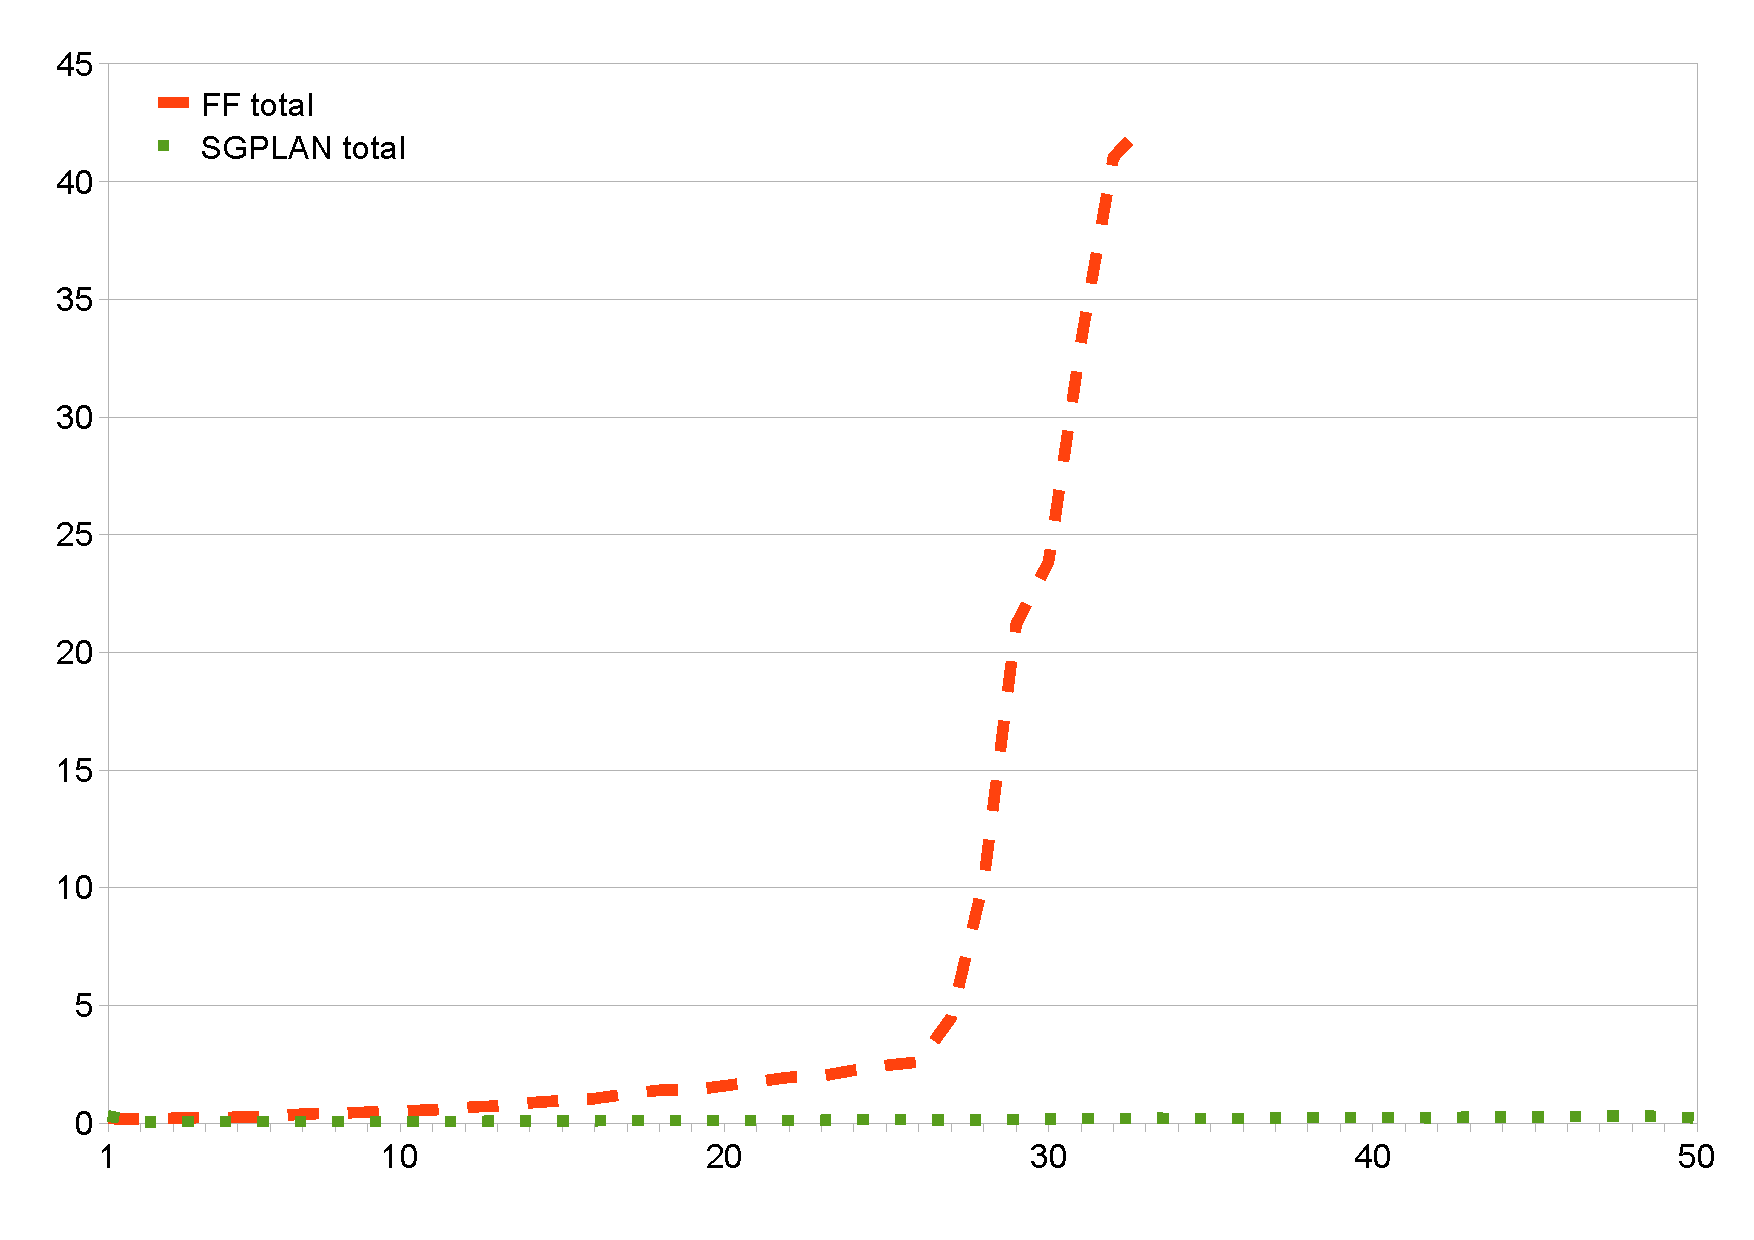
\includegraphics[width=0.85\columnwidth]{graph-exp4}
  %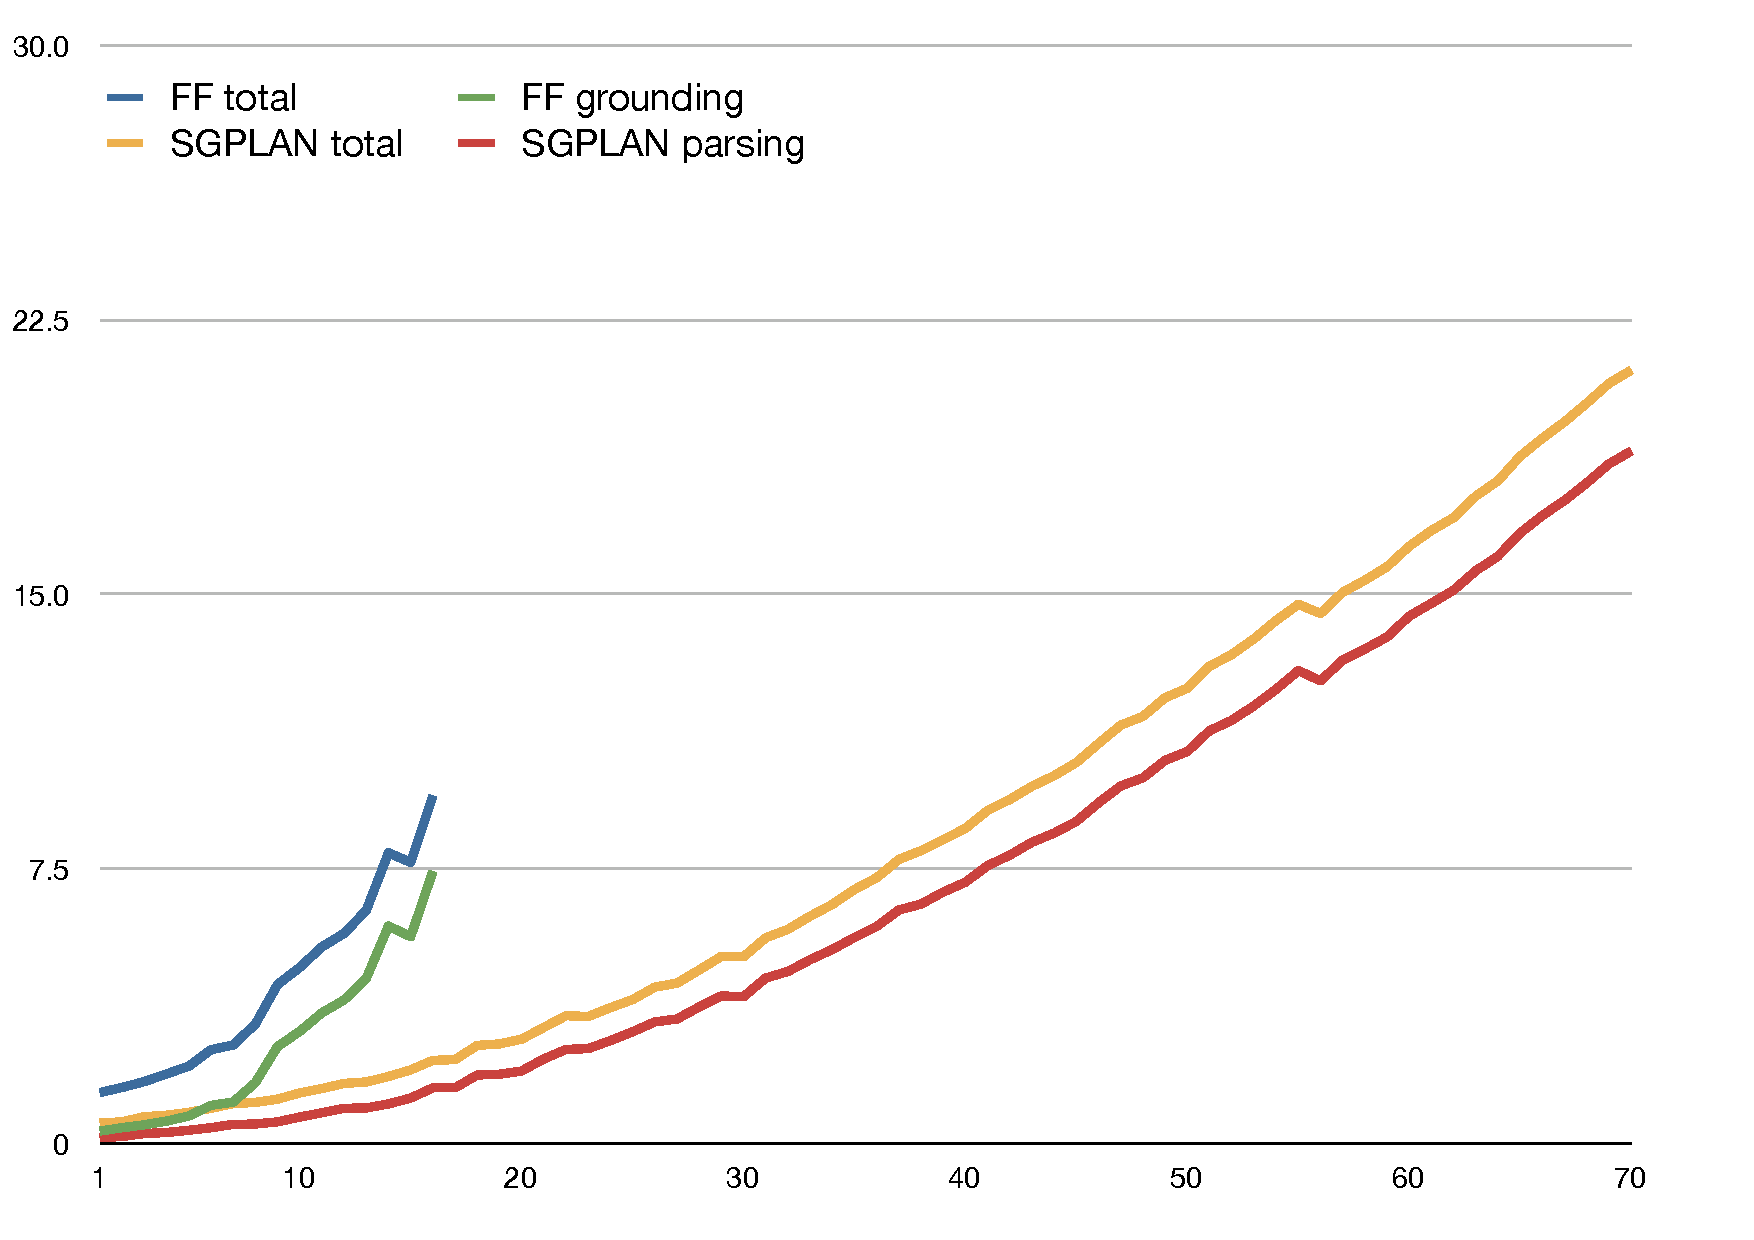
\includegraphics[width=1\columnwidth]{pic-runtime-empty-world}
  \caption{Results on the GIVE domain with inaccessible
    positions for $h=20$ and $n=5$. The horizontal axis is $w$.
    The vertical axis is the runtime in seconds.}
  \label{fig:give-runtime-nosoln}
\end{figure}



%%% Local Variables: 
%%% mode: latex
%%% TeX-master: "manuscript"
%%% End: 
